\documentclass[12pt,twoside]{article}   
\usepackage{../../light}

\newcommand{\hint}[1]{({\it Hint: #1})}
\newcommand{\card}[1]{\left|#1\right|}
\newcommand{\union}{\cup}
\newcommand{\lgunion}{\bigcup}
\newcommand{\intersect}{\cap}
\newcommand{\lgintersect}{\bigcap}
\newcommand{\cross}{\times}

\hidesolutions
\showsolutions

\newlength{\strutheight}
\newcommand{\prob}[1]{\mathop{\textup{Pr}} \nolimits \left( #1 \right)}
\newcommand{\prsub}[2]{\mathop{\textup{Pr}_{#1}}\nolimits\left(#2\right)}
\newcommand{\prcond}[2]{%
  \ifinner \settoheight{\strutheight}{$#1 #2$}
  \else    \settoheight{\strutheight}{$\displaystyle#1 #2$} \fi%
  \mathop{\textup{Pr}}\nolimits\left(
    #1\,\left|\protect\rule{0cm}{\strutheight}\right.\,#2
  \right)}
\newcommand{\comment}[1]{}
\newcommand{\cE}{\mathcal{E}}
\renewcommand{\setminus}{-}
\renewcommand{\complement}[1]{\overline{#1}}


\begin{document}
\problemset{12}{November 29, 2016}{Monday, December 5, 7:30 pm}
\noindent \textbf{Reading Assignment:}   Sections  16.1 - 16.5

%%%%%%%%%%%%%%%%%%%%%%%%%%%%%%%%%%%%%%%%%%%%%%%%%%%%%%%%%%%%%%%%%%%%%%%%%%%%%
%%% Fall07 ps10 problem 1


%%%%%%%%%%%%%%%%%%%%%%%%%%%%%%%%%%%%%%%%%%%%%%%%%%%%%%%%%%%%%%%%%%%%%%%%%%%%%%
%
%\begin{problem}{20} \textit{Finalphobia} is a rare
%disease in which the victim has the delusion that he or she is being
%subjected to an intense mathematical examination.
%%
%\begin{itemize}
%\item A person selected uniformly at random has finalphobia with probability
%$1/100$.
%\item A person with finalphobia has shaky hands with probability $9/10$.
%\item A person without finalphobia has shaky hands with probability $1/20$.
%\end{itemize}
%%
%What is the probablility that a person selected uniformly at random
%has finalphobia, given that he or she has shaky hands?
%
%\solution{
%Let $F$ be the event that the randomly-selected person has
%finalphobia, and let $S$ be the event that he or she has shaky hands.
%A tree diagram is worked out below:
%%
%\begin{center}
%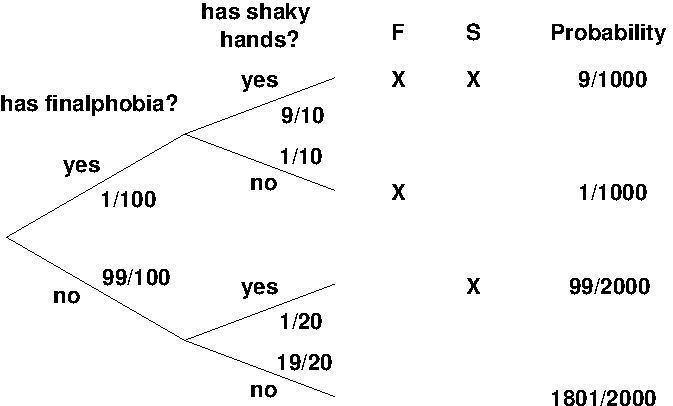
\includegraphics{finalphobia}
%\end{center}
%%
%The probability that a person has finalphobia, given that he or she
%has shaky hands is:
%%
%\begin{align*}
%\prcond{F}{S}
%    & = \frac{\pr{F \cap S}}{\pr{S}} \\
%        & = \frac{9/1000}{9/1000 + 99/2000} \\
%	    & = \frac{18}{18+99} \\
%	        & = \frac{18}{117}
%\end{align*}
%
%So, while it's true that someone with shaky hands is five times more likely to have finalphobia than someone with steady hands, it remains a poor bet---about 1 in 5---that someone with shaky hands actually has does have finalphobia.}
%
%\end{problem}


%%%%%%%%%%%%%%%%%%%%%%%%%%%%%%%%%


%%%%%%%%%%%%%%%%%%%%%%%%%%%%%%%%%%%%%%%%%%%%%%%%%%%%%%%%%

%%%%%%%%%%%%%%%%%%%%%%%%%

\begin{problem}{15}
In lecture we discussed the Birthday Paradox. Namely, we found that in a group of $m$ people with $N$ possible birthdays, if $m \ll N$, then:
\[
\pr{\text{all $m$ birthdays are different}} \sim e^{-\frac{m(m-1)}{2N}}
\]
To find the number of people, $m$, necessary for a half chance of a match, we set the probability to $1/2$ to get:
\[
m \sim \sqrt{(2\ln2)N} \approx 1.18\sqrt{N}
\]

For $N = 365$ days we found $m$ to be 23.

We could also run a different experiment. As we put on the board the birthdays of the poeple surveyed, we could ask the class if anyone has the same birthday. In this case, before we reached a match amongst the surveyed people, we would already have found other people in the rest of the class who have the same birthday as someone already surveyed. Let's investigate why this is.

\bparts
\ppart{5} Consider a group of $m$ people with $N$ possible birthdays amongst a larger class of $k$ people, such that $m \leq k$. Define $\pr{A}$ to be the probability that $m$ people all have different birthdays \textit{and} none of the other $k-m$ people have the same birthday as one of the $m$.

Show that, if $m \ll N$, then $\pr{A} \sim e^{\frac{m(m-2k)}{2N}}$. (Notice that the probability of no match is $e^{-\frac{m^2}{2N}}$ when $k$ is $m$, and it gets smaller as $k$ gets larger.)

\hspace{0.5in} \textit{Hints:} For $m \ll N$: $\frac{N!}{(N-m)!N^m} \sim e^{-\frac{m^2}{2N}}$, and $(1-\frac{m}{N}) \sim e^{-\frac{m}{N}}$.

\solution{
We know:
\[
\pr{A} = \frac{N(N-1)\ldots(N-m+1)\cdot(N-m)^{k-m}}{N^k}
\]

since there are $N$ choices for the first birthday, $N-1$ choices for the second birthday, etc., for the first $m$ birthdays, and $N-m$ choices for each of the remaining $k-m$ birthdays. There are total $N^k$ possible combinations of birthdays within the class.

\begin{align*}
\pr{A} &= \frac{N(N-1)\ldots(N-m+1)\cdot(N-m)^{k-m}}{N^k} \\
&= \frac{N!}{(N-m)!}\left(\frac{(N-m)^{k-m}}{N^k}\right) \\
&= \frac{N!}{(N-m)!N^m}\left(\frac{N-m}{N}\right)^{k-m} \\
&= \frac{N!}{(N-m)!N^m}\left(1-\frac{m}{N}\right)^{k-m} \\
&\sim e^{-\frac{m^2}{2N}} \cdot e^{-\frac{m}{N}(k-m)} & \text{(by the Hint)} \\
& = e^{\frac{m(m-2k)}{2N}}
\end{align*}
}

\ppart{10} Find the approximate number of people in the group, $m$, necessary for a half chance of a match (your answer will be in the form of a quadratic). Then simplify your answer to show that, as $k$ gets large  (such that $\sqrt{N} \ll k$), then $m \sim \frac{N\ln2}{k}$.

\hspace{0.5in} \textit{Hint:} For $x \ll 1$: $\sqrt{1-x} \sim (1-\frac{x}{2})$.

\solution{
Setting $\pr{A} = 1/2$, we get a solution for $m$:

\begin{align*}
1/2 &= e^{\frac{m(m-2k)}{2N}} \\
-2N\ln2 &= m^2 -2km  \\
0 &= m^2-2km + (2N\ln2) \\
m &= \frac{2k \pm \sqrt{(2k)^2 - 4(2N\ln2)}}{2}
\end{align*}

Simplifying the solution under the assumption of large $k$, we find:
\begin{align*}
m &= \frac{2k - \sqrt{4k^2 - 8N\ln2}}{2} & \text{(taking the lower positive root)} \\
&= k - k\sqrt{1 - \frac{2N\ln2}{k^2}} \\
&\sim k  - k \left(1-\frac{2N\ln2}{2k^2}\right) & \text{(by the Hint)} \\
&= \frac{N\ln2}{k}  
\end{align*}
}

\eparts

\end{problem}

%%%%%%%%%%%%%%%%%%%%%%%%%

\begin{problem}{10}
Suppose that events $A, B, C, D$ are mutually independent.  Prove whether each of the following statements is true or give a counterexample if it is false.

\bparts
\ppart{5} $A \cap C$ is independent of $\bar{B} \cap D$ where $\bar{B}$ denotes the complement of $B$.
\solution{
This statement is true.  Intuitively, knowing that events $A$ and $C$ occurred should tell you nothing about events $\bar{B}$ and $D$ occurring.  More formally, 

\begin{equation*}
\begin{split}
p(A \cap \bar{B} \cap C \cap D) + p(A \cap B \cap C \cap D) &= p(A \cap C \cap D) \\
\implies p(A \cap \bar{B} \cap C \cap D) &= p(A) \cdot p(C) \cdot p(D) (1 - p(B)) \\
\implies p(A \cap \bar{B} \cap C \cap D) &= p(A \cap C) \cdot p(\bar{B} \cap D) \\
\end{split}
\end{equation*}
}

\ppart{5} $A \cap \bar{B} \cap C$ is independent of $\bar{B} \cup \bar{C}$.
\solution{
This statement is false.  Intuitively, knowing that event $A \cap \bar{B} \cap C$ occurred implies that $C$ occurred and so this influences the probability that $\bar{B} \cup \bar{C}$ occurs.  As a counterexample, consider 4 independent coin tosses, and let $A$ be the event that the first coin is a heads, $B$ the event that the second coin is a heads, $C$ be the event that the third coin is a heads, and $D$ be the event that the fourth coin is a heads.  Now $p(A \cap \bar{B} \cap C) = \frac{1}{8}$ and $p(\bar{B} \cup \bar{C}) = 1 - \frac{1}{4} = \frac{3}{4}$.  Finally,

\begin{equation*}
\begin{split}
p((A \cap \bar{B} \cap C) \cap (\bar{B} \cup \bar{C})) &= p((A \cap \bar{B} \cap C \cap \bar{B}) \cup (A \cap \bar{B} \cap C \cap \bar{C})) \\
&= p(A \cap \bar{B} \cap C) \\
&= \frac{1}{8} \\
\end{split}
\end{equation*}

Now since $p((A \cap \bar{B} \cap C) \cap (\bar{B} \cup \bar{C}))  \neq p(A \cap \bar{B} \cap C) \cdot p(\bar{B} \cup \bar{C})$, these events are not independent.

}

\eparts
\end{problem}
\begin{problem}{20}

You roll 2 five-sided die.  The sides of each die are numbered from 1 to 5.  All sides of each die have an equal probability of appearing, and the two die rolls are independent.  Let event $A$ be that sum of the results of the rolls of the two die is 10, and let $B$ be the event that the sum of the results of the rolls of the two die is 8.  

\bparts

\ppart{5} Is $A$ independent of the event that at least one of the die rolls resulted in a 5?

\solution{
No.  $p(A) = \frac{1}{25}$.  Let $F$ be the event that at least one of the die rolls resulted in a 5.  Then $p(F) = \frac{5}{25} + \frac{5}{25} - \frac{1}{25} = \frac{9}{25}$.  Finally $p(A \cap F) = \frac{1}{25}$ since if event $A$ happens then both die rolls must have resulted in a 5. Now as $p(A \cap F) \neq p(A) \cdot p(F)$, the events are not independent.
}

\ppart{5} Is $A$ independent of the event that at least one of the die rolls resulted in a 3?

\solution{
No.  Again $p(A) = \frac{1}{25}$.  Now let $T$ be the event that at least one of the die rolls resulted in a $3$.  $p(T) = \frac{9}{25}$ as before.  However $p(A \cap T) = 0$ since both die rolls need to result in a 5 for event $A$ to happen.
}

\ppart{5} Is $B$ independent of the event that both die rolls resulted in the same number?

\solution{
No.  $p(B) = \frac{3}{25}$.  Let $S$ be the event that both die rolls resulted in the same number.  Then $p(S) = \frac{5}{25}$.  Now $p(B \cap S) = \frac{1}{25}$, which is not equal to $\frac{3}{25} \cdot \frac{5}{25}$.   
}

\ppart{5} Is $B$ independent of the event that at least one of the die rolled a 3?
\solution{
No.  Again $p(B) = \frac{3}{25}$.  Now let $T$ be the event that at least one of the die rolled a 3.  Then $p(T) = \frac{9}{25}$.  Now, $p(B \cap T) = \frac{2}{25}$, which is not equal to $\frac{3}{25} \cdot \frac{9}{25}$.  
}
\eparts

\end{problem}

%%%%%%%%%%%%%%%%%%%%%%%%%
%% Spring08, Pset 11, Problem 7
\begin{problem}{20}

\bparts

\ppart{5} Suppose $A$ and $B$ are \emph{disjoint} events.  Prove that $A$ and
$B$ are \emph{not independent}, unless $\prob{A}$ or $\prob{B}$ is zero.

\solution{ Since $A$ and $B$ are disjoint, 
\[
\prob{A \intersect B} =  \prob{\emptyset}  = 0.
\]
So, $\prob{A \intersect B}=\prob{A} \cdot \prob{B}$ iff $\prob{A}=0$ or $\prob{B}=0$.
}


\ppart{5} If $A$ and $B$ are independent, prove that $A$ and $\bar{B}$
are also independent.

\textit{Hint:  $\prob{A \intersect \bar{B}} = \prob{A} - \prob{A \intersect B}$.}

\iffalse

You may find it useful to use results from Problem
\ref{Identities}.

Problem \ref{Identities} (\ref{setminus})
\fi

\solution{
\begin{align*}
\prob{A \intersect \bar{B}}
% &= \prob{A - B} \\
 &= \prob{A} - \prob{A \intersect B} &&\text{(by the hint)} \\
 &= \prob{A} - \prob{A} \cdot \prob{B} &&\text{(since $A$ and $B$ are independent)} \\
 &= \prob{A} \cdot (1 - \prob{B}) \\
 &= \prob{A} \cdot \prob{\bar{B}}.
\end{align*}
The last equality holds since the probability of any event equals $1$ minus the probability of its
complement.
Thus, we have shown that $\prob{A \intersect \bar{B}}=\prob{A} \cdot \prob{\bar{B}}$,
which is equivalent to $A$ and $\bar{B}$ being independent.
}


\ppart{5} 
Give an example of events $A$,$B$, $C$ such that $A$ is independent of $B$,
$A$ is independent of $C$, but $A$ is not independent of $B\union C$.

\solution{The experiment is 2 independent coin flips, letting $A$ be ``the
1st flip is heads'', $B$ the ``the 2nd flip is heads,'' $C$ is ``odd
number of heads.''  Then $A$ is not independent of $B \union C$ because
\[
\prcond{A}{B \union C}= \frac{\prob{A \intersect (B \union C)}}{\prob{B \union C}}= \frac{\prob{HH,HT}}{\prob{HH,TH,HT}} = 2/3 \neq 1/2 = \prob{A}.
\]

\iffalse

Consider the usual random experiment of
rolling a die and let $A$, $B$, $C$ be the events that the die rolls
less than 3, rolls an even number, or rolls a prime number,
respectively. I.e., 
\[
A = \{1,2\} \qquad
B = \{2,4,6\} \qquad
C = \{2,3,5\}.
\]
Then, 
$$
\prob{A}=\tfrac{1}{3}, 
\qquad
\prob{B}=\prob{C}=\tfrac{1}{2},
$$
and
$$
\prob{A\cap B}=
\prob{A\cap C}=
\prob{B\cap C}=
\prob{A\cap B\cap C}=
\prob{\{2\}}=
\tfrac{1}{6}.
$$
Easily, 
$$
\prob{A\mid B}=
\prob{A\mid C}=
\tfrac{1}{6}/\tfrac{1}{2}=
\tfrac{1}{3}=
\prob{A},
$$
which proves $A$ is independent of $B$ and also independent of
$C$. However, 
$$
\prob{A\mid B\cap C}=
\prob{A\cap B\cap C}/\prob{B\cap C}=
\tfrac{1}{6}/\tfrac{1}{6}=
1\neq
\prob{A},
$$
which implies $A$ is not independent of $B\cap C$.
\fi

}

\ppart{5} Prove that if $C$ is independent of $A$, and $C$ is independent of
$B$, and $C$ is independent of $A \intersect B$, then $C$ is independent
of $A \union B$.

\textit{Hint:} Calculate $\prcond{A \union B}{C}$.

\solution{
Conditional inclusion-exclusion followed by plain inclusion-exclusion provides
a quick proof:
\begin{align*}
\prcond{A \union B}{C}
 &= \prcond{A}{C} + \prcond{B}{C} - \prcond{A \intersect B}{C}
    & \text{(by conditional inc-ex)}\\
 &= \prob{A} + \prob{B} - \prob{A \intersect B}
    &\text{(by independence)} \\
 &= \prob{A \union B}
    & \text{(by regular inc-ex)}
\end{align*}
}
\eparts
\end{problem}

%%%%%%%%%%%%%%%%%%%%%%%%%%%%%%%%%%%%%%%%%%%%%%%%%%%%%%%%%%
\begin{problem}{20}

  Professor Moitra has a deck of $52$ randomly shuffled playing cards, $26$ red, $26$ black.  He proposes the following game: he will continually draw a card off the top of the deck and turn it face up so that you can see it and then put it aside.  At any point while there are still cards left in the deck, you may choose to stop and he will flip over one last card.  If the next card turns up black you win and otherwise you lose.  Either way, the game ends.

\bparts

\ppart{4} Show that if you choose to stop before you have seen any
cards, you then have probability $1/2$ of winning the game.

\solution{If we just record the sequence of black and red cards that
  will be drawn, there are $\binom{51}{25}$ sequences with first card
  black: $25$ positions for the black cards chosen from the $51$
  remaining positions.  Since there are $\binom{52}{26}$ sequences in
  all, the probability of winning on the first draw is
  $\binom{51}{25}/\binom{52}{26} = 26/52 = 1/2$.}

\ppart{4} Suppose you don't choose to stop before the first card is flipped and it turns up red. Show that you have then have a probability of winning the game that is
greater than $1/2$.

\solution{Suppose you take the next card after that.  There are
  $\binom{50}{25}$ sequences that start with a red card and then a
  black and there are $\binom{51}{26}$ sequences that start with a red
  card. So then there is a $\binom{50}{25}/\binom{50}{26} = 26/51 >
  1/2$ chance of winning.  Any optimum strategy would have to
  guarantee a probability of winning as least as big as that.}

\ppart{4} If there are $r$ red cards left in the deck and $b$ black
cards, show that the probability of winning if you choose to stop before the next card
is flipped is $b/(r+b)$.

\solution{The probability is $\binom{b+r-1}{b-1}/\binom{b+r}{b} =
b/(r+b)$.}


\ppart{8} Either,
\begin{enumerate}
\item come up with a strategy for this game that gives you a
  probability of winning strictly greater than $1/2$ and prove that
  the strategy works, or,
\item come up with a proof that no such strategy can exist.
\end{enumerate}

\solution{There is no such strategy.  Let $S_{b,r}$ be a strategy that
  acchieves the best probability of winning when starting with $b$
  black cards and $r$ red cards.  The claim is that $\Pr(\mbox{win by
    playing $S_{b,r}$}) = b/(r+b)$ for all $b,r$ with at least $b>0$
  or $r>0$.

  Clearly $\Pr(\mbox{win by playing $S_{1,0}$}) = 1$ and
  $\Pr(\mbox{win by playing $S_{0,1}$}) = 0$. We prove the rest of the
  claim by induction on $r+b$.  If the strategy $S_{b,r}$ is to take
  the next card, then $\Pr(\mbox{win by playing $S_{b,r}$}) = b/(r+b)$
  as claimed.  Suppose then that the strategy $S_{r,b}$ is to not take
  the first card, but to keep playing.  Then the first card is going to be red with probability $r/(r+b)$ and it's going to be black with probability $b\
/(r+b)$.  If the first card is black then we now have $b-1$ black cards remaining and $r$ red cards remaining and we should play $S_{b-1,r}$ which by ou\
r inductive hypothesis has a probability of $(b-1)/(b+r-1)$ of winning. On the other hand, if the first card is red, we now have $r-1$ red cards and $b$\
 black cards remaining and we should play $S_{b,r-1}$ which by our inductive hypothesis has a probability of $b/(b+r-1)$ of winning. This gives us a tot\
al probability of  \[\Pr(\mbox{win by playing $S_{b,r}$}) = ((b-1)/(b-1+r))(b/(r+b)) +  (b/(b+r-1))(r/(b+r)) = b/(b+r),\] as claimed.  This is summarize\
d in the diagram below.

\begin{center}
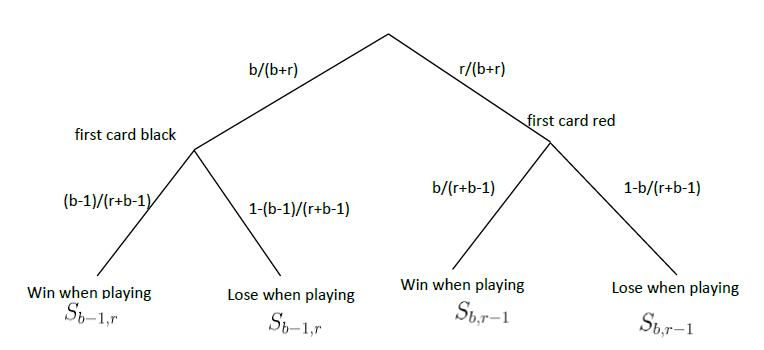
\includegraphics[width = 150mm]{last_problem.jpg}
\end{center}

}
\eparts

\end{problem}

%%%%%%%%%%%%%%%%%%%%%%%%%%%%%%%%%%%%%%%%%%%%%%%%%%%%%%%%%%
%New problem
\begin{problem}{15}
Three very rare DNA markers were found in the DNA collected at a crime scene. Only one in every $1,000$ people has marker $A$, one in every $3,000$ people has marker $B$, and one in every $5,000$ people has marker $C$. Joe the plumber was arrested and accused of committing the crime, because he had all those markers present in his DNA. The prosecutor argues that the chances of any person having all three DNA markers is \[\frac1{1000}\cdot\frac{1}{3000}\cdot \frac1{5000} = \frac{1}{15,000,000,000}\], which is more than $1$ over the number of people in the world. This, plus the fact that Joe the plumber lives only 100 miles away from the crime scene must clearly mean that he is guilty. Having taken $6.042$, you should be suspicious of this reasoning.
\bparts
\ppart{2}
What assumption has the prosecutor made (even though he hasn't realized it) about the presence of the $3$ markers in human DNA?
\solution{Mutual independence.}
\ppart{4}
What would be the probability of a person having all three markers assuming that the markers appear pairwise independently? Under this assumption, can it be stated with such certainty that Joe the plumber commited the crime?
\solution{\[Pr[A\intersect B \intersect C] \leq Pr[B \intersect C] = Pr[B]\cdot Pr[C] = \frac{1}{15,000,000}\]
One in $15,000,000$ people might have all the three markers, and the fact that Joe the plumber lives $100$ miles away means nothing if the crime was committed in, say, New York City.}
\ppart{4}
What can you say about the probability of a person having all three markers if there is no independence between the markers?
\solution{The probability is at most \[P[C] = \frac{1}{5,000}.\]}
\ppart{5}
In fact, it turns out that neither of the above assumptions is correct. A researcher from MIT (who was actually in your recitation section for 6.042 back in the day) has discovered that while markers B and C appear independently, the probability of having marker B if you have marker A is $\frac12$ and the probability of having marker C if you have marker A is $\frac13$. The defence attorney now argues that the probability of a randomly selected person having all three markers is 
\[Pr[A\intersect B\intersect C] = Pr[A]\cdot Pr[B|A] \cdot Pr[C|A] =  \frac{1}{1000} \cdot \frac12 \cdot \frac13 = \frac{1}{6,000}.\]
Called as a witness, the MIT researcher points out that this is not necessarily true and that in fact he himself does not know what the probability is. What is wrong with the defence attorney's reasoning? (We assume that the MIT researcher published correct information and that, since he took 6.042, he knows what he is talking about.)
\solution{The researcher said that markers B and C appear independently, but he never said that they are independent if the person has marker A.}
\eparts
\end{problem}

\end{document}